\begin{flushright} {\tiny {\color{gray} \tt (tikz\_q1.tex)}} \end{flushright}
%~~~~~~~~~~~~~~~~~~~~~~~~~~~~~~~~~~~~~~~~~~~~~~~~~~~~~~~~~~~~~~~~~~~~~~~~~~~~~~~~~~~~~~~~~~~~~~~~~~

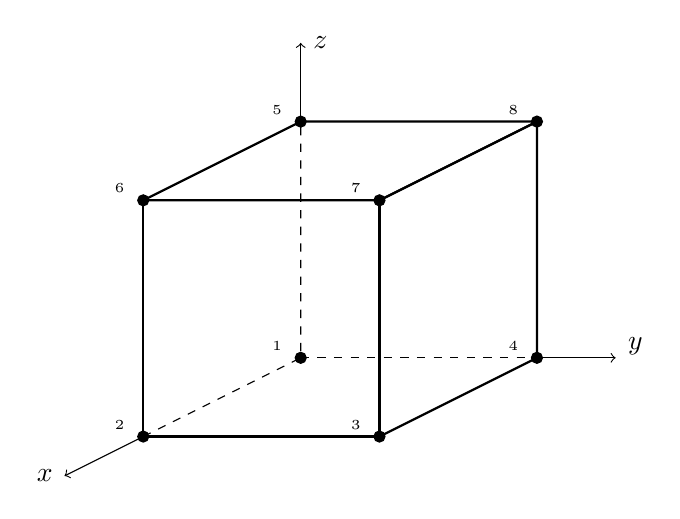
\begin{tikzpicture}
%\draw[fill=gray!23,gray!23](0,0) rectangle (9,7);
%\draw[step=0.5cm,gray,very thin] (0,0) grid (9,7); %background grid

\draw[thick] (2,4.5) -- (5,4.5) -- (7,5.5) -- (4,5.5) -- cycle; %top
\draw[thick] (2,1.5) -- (5,1.5) -- (5,4.5) -- (2,4.5) -- cycle; %front
\draw[thick] (5,1.5) -- (7,2.5) -- (7,5.5) -- (5,4.5) -- cycle; %right

\draw[dashed]   (2,1.5) -- (4,2.5) -- (4,5.5) ; % 
\draw[dashed]   (4,2.5) -- (7,2.5)  ; % 

\draw[thin,->] (2,1.5) -- (1,1); %x
\draw[thin,->] (7,2.5) -- (8,2.5); %y
\draw[thin,->] (4,5.5) -- (4,6.5); %z
\node[] at (0.75,1) {$x$};
\node[] at (8.25,2.65) {$y$};
\node[] at (4.25,6.5) {$z$};

\draw[black,fill=black] (4,2.5)   circle (2pt);
\draw[black,fill=black] (2,1.5)   circle (2pt);
\draw[black,fill=black] (7,2.5)   circle (2pt);
\draw[black,fill=black] (5,1.5)   circle (2pt);
\draw[black,fill=black] (4,5.5)   circle (2pt);
\draw[black,fill=black] (2,4.5)   circle (2pt);
\draw[black,fill=black] (7,5.5)   circle (2pt);
\draw[black,fill=black] (5,4.5)   circle (2pt);

\node[] at (3.7,2.65) {\tiny 1};
\node[] at (1.7,1.65) {\tiny 2};
\node[] at (6.7,2.65) {\tiny 4};
\node[] at (4.7,1.65) {\tiny 3};

\node[] at (3.7,5.65) {\tiny 5};
\node[] at (1.7,4.65) {\tiny 6};
\node[] at (6.7,5.65) {\tiny 8};
\node[] at (4.7,4.65) {\tiny 7};
\end{tikzpicture}

